\documentclass{../../slides-style}

\slidetitle{Списки}{13.10.2023}

\begin{document}
	
	\begin{frame}[plain]
        \titlepage
    \end{frame}
	
	\begin{frame}
		\frametitle{Список}
		\begin{columns}
			\begin{column}{0.55\textwidth}
				\begin{itemize}
					\item Элементы можно добавлять и удалять в произвольной позиции
					\item Используется для
					\begin{itemize}
						\item Замены массиву, когда количество данных неизвестно
						\item Когда требуется часто добавлять и удалять элементы в произвольной позиции
					\end{itemize}
				\end{itemize}
			\end{column}
			\begin{column}{0.45\textwidth}
				\begin{center}
					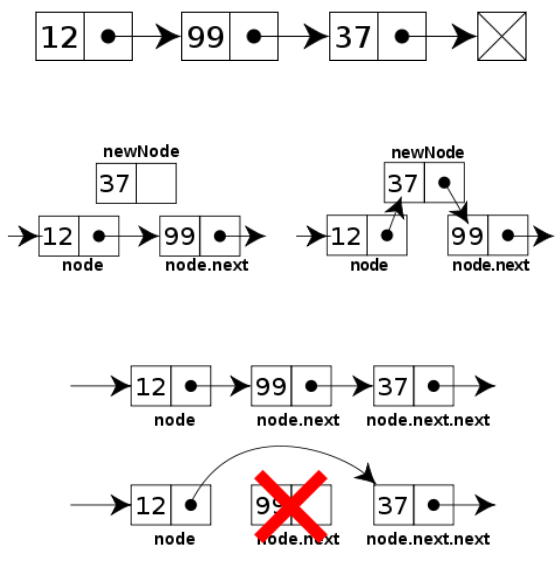
\includegraphics[width=0.95\textwidth]{list.png}
				\end{center}
			\end{column}
		\end{columns}
	\end{frame}

	\begin{frame}
		\frametitle{Двусвязный список}
		\begin{itemize}
			\item Нет проблем с определением позиции
			\item Позволяет ходить в прямом и обратном направлении
			\item Несколько сложнее в реализации
			\item Требует несколько больше памяти
			\begin{center}
				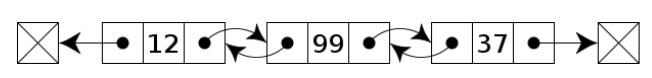
\includegraphics[width=0.75\textwidth]{double-linked-list.png}
			\end{center}
		\end{itemize}
	\end{frame}

	\begin{frame}
		\frametitle{Циклический список}
		\begin{itemize}
			\item Особо не нужен, но прикольно
			\item При удалении произвольного элемента надо проверить, не голова ли это
			\begin{center}
				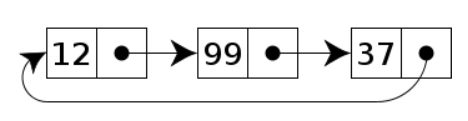
\includegraphics[width=0.45\textwidth]{cyclic-list.png}
			\end{center}
		\end{itemize}
	\end{frame}
	

\end{document}